% !TEX root = Simulation.tex

\chapter{Fractals - Text Chapter 7}

\section{Problem 10}
\textbf{
Implement a bracketed OL-system and reproduce all plant-like structures of Figure~7.24 in the text. Change some derivation rules and see what happens. Make your own portfolio with at least ten plants.
}

\hfill \\

The first step to solving this problem was to gather the necessary test input. The parameters from Figure~7.24 in the text were summarized into Figure~\ref{7.24_rep}. The images were created using the program developed for the problem.

After collecting the necessary data, I saw two distinct parts to this problem. One was to create the L-system strings, and the other was to interpret them using Python's Turtle graphics (as suggested).

\subsection{L-system generation}
L-systems are rather straight forward so I made a simple class to encapsulate them. I tested this class against the example in section 7.4.3 in the text. The results can be found in Figure~\ref{lsystem_results}.

\begin{figure}
\centering
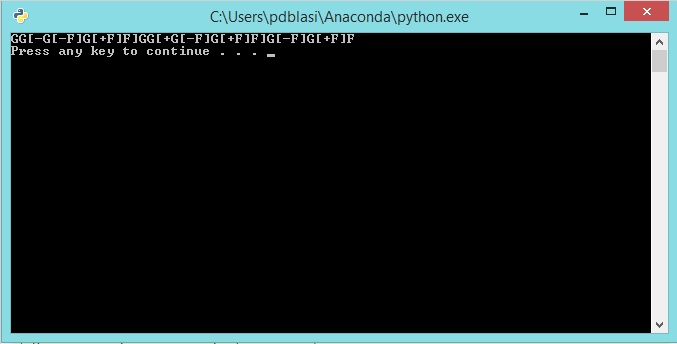
\includegraphics[scale=.75]{LSystemResults}
\caption{LSystem Results}
\label{lsystem_results}
\end{figure}


\subsection{Turtle Graphics representation}

\begin{figure}
\centering
\begingroup \everymath{\scriptstyle}
\begin{tabular}{ | c | c | c | }
\hline
IMAGE1 & IMAGE2 & IMAGE3 \\

$\begin{aligned}
& t = 8, \delta = 22.5\degree \\
& \omega = G \\
& G \rightarrow F+[[G]-G]-F[-FG]+G \\
& F \rightarrow FF
\end{aligned}$ & 
$\begin{aligned}
& t = 4, \delta = 22.5\degree \\
& \omega = F \\
& F \rightarrow FF+[+F-F-F]-[-F+F+F]
\end{aligned}$ & 
$\begin{aligned}
& t = 6, \delta = 22.5\degree \\
& \omega = G \\
& G \rightarrow F[+FFG][G]-FG \\
& F \rightarrow FF
\end{aligned}$ \\ \hline

IMAGE4 & IMAGE5 & IMAGE6 \\

$\begin{aligned}
& t = 9, \delta = 20\degree \\
& \omega = G \\
& G \rightarrow F[-G]F[+G]-G \\
& F \rightarrow FF
\end{aligned}$ &
$\begin{aligned}
& t = 9, \delta = 25.7\degree \\
& \omega = G \\
& G \rightarrow F[-G][+G]FG \\
& F \rightarrow FF
\end{aligned}$ &
$\begin{aligned}
& t = 5, \delta = 22.5\degree \\
& \omega = G \\
& G \rightarrow FG[-F[G]-G][G+G][+F[G]+G] \\
& F \rightarrow FF
\end{aligned}$ \\ \hline
\end{tabular}
\endgroup
\caption{Reproduction of figure 7.24 in the text}
\label{7.24_rep}
\end{figure}

\section{Problem 15}
\textbf{
Implement a recursive iterated function system (RIFS) to generate all the fractals whose codes are presented in Table~7.3 in the text.
}

\hfill \\

Again, the first step was to reproduce the data needed for the problem. Table~7.3 from the text has been reproduced in Table~\ref{7.3_rep}

\begin{table}
\begin{tabular}{ c c }
	\begin{tabular}{ c c c c c c c c }
	\hline
	w & a & b & c & d\footnote{Corrected as suggested on assignment page} & e & f & p \\
	\hline
	1 & 0.5 & 0 & 0 & 0.5 & 1 & 1 & 0.33 \\
	2 & 0.5 & 0 & 0 & 0.5 & 1 & 50 & 0.33 \\
	3 & 0.5 & 0 & 0 & 0.5 & 50 & 50 & 0.34 \\
	\hline
	\multicolumn{8}{c}{Sierpinski Gasket}
	\end{tabular} &

	\begin{tabular}{ c c c c c c c c }
	\hline
	w & a & b & c & d & e & f & p \\
	\hline
	1 & 0.5 & 0 & 0 & 0.5 & 1 & 1 & 0.25 \\
	2 & 0.5 & 0 & 0 & 0.5 & 50 & 1 & 0.25 \\
	3 & 0.5 & 0 & 0 & 0.5 & 1 & 50 & 0.25 \\
	4 & 0.5 & 0 & 0 & 0.5 & 50 & 50 & 0.25 \\
	\hline
	\multicolumn{8}{c}{Square}
	\end{tabular} \\
	
	\hfill & \hfill \\
	
	\begin{tabular}{ c c c c c c c c }
	\hline
	w & a & b & c & d & e & f & p \\
	\hline
	1 & 0 & 0 & 0 & 0.16 & 0 & 0 & 0.01 \\
	2 & 0.85 & 0.04 & -0.04 & 0.85 & 0 & 1.6 &0.85 \\
	3 & 0.2 & -0.26 & 0.23 & 0.22 & 0 & 1.6 & 0.07 \\
	4 & -0.15 & 0.28 & 0.26 & 0.24 & 0 & 0.44 & 0.07 \\
	\hline
	\multicolumn{8}{c}{Barnsley Fern}
	\end{tabular} &
	
	\begin{tabular}{ c c c c c c c c }
	\hline
	w & a & b & c & d & e & f & p \\
	\hline
	1 & 0 & 0 & 0 & 0.5 & 0 & 0 & 0.05 \\
	2 & 0.42 & -0.42 & 0.42 & 0.42 & 0 & 0.2 & 0.40 \\
	3 & 0.42 & 0.42 & -0.42 & 0.42 & 0 & 0.2 & 0.40 \\
	4 & 0.1 & 0 & 0 & 0.1 & 0 & 0.2 & 0.15 \\
	\hline
	\multicolumn{8}{c}{Tree}
	\end{tabular}
\end{tabular}
\caption{Reproduction of Table 7.3 from the text}
\label{7.3_rep}
\end{table}

\section{Problem 21}
\textbf{
Implement the random midpoint displacement algorithm in 3D and generate some fractal landscapes. Study the influence of H on the landscapes generated.
}

\hfill \\
